\documentclass[]{article}
\usepackage{lmodern}
\usepackage{amssymb,amsmath}
\usepackage{ifxetex,ifluatex}
\usepackage{fixltx2e} % provides \textsubscript
\ifnum 0\ifxetex 1\fi\ifluatex 1\fi=0 % if pdftex
  \usepackage[T1]{fontenc}
  \usepackage[utf8]{inputenc}
\else % if luatex or xelatex
  \ifxetex
    \usepackage{mathspec}
  \else
    \usepackage{fontspec}
  \fi
  \defaultfontfeatures{Ligatures=TeX,Scale=MatchLowercase}
\fi
% use upquote if available, for straight quotes in verbatim environments
\IfFileExists{upquote.sty}{\usepackage{upquote}}{}
% use microtype if available
\IfFileExists{microtype.sty}{%
\usepackage{microtype}
\UseMicrotypeSet[protrusion]{basicmath} % disable protrusion for tt fonts
}{}
\usepackage[margin=1in]{geometry}
\usepackage{hyperref}
\hypersetup{unicode=true,
            pdftitle={hw\_01},
            pdfauthor={Abby Bergman},
            pdfborder={0 0 0},
            breaklinks=true}
\urlstyle{same}  % don't use monospace font for urls
\usepackage{color}
\usepackage{fancyvrb}
\newcommand{\VerbBar}{|}
\newcommand{\VERB}{\Verb[commandchars=\\\{\}]}
\DefineVerbatimEnvironment{Highlighting}{Verbatim}{commandchars=\\\{\}}
% Add ',fontsize=\small' for more characters per line
\usepackage{framed}
\definecolor{shadecolor}{RGB}{248,248,248}
\newenvironment{Shaded}{\begin{snugshade}}{\end{snugshade}}
\newcommand{\KeywordTok}[1]{\textcolor[rgb]{0.13,0.29,0.53}{\textbf{#1}}}
\newcommand{\DataTypeTok}[1]{\textcolor[rgb]{0.13,0.29,0.53}{#1}}
\newcommand{\DecValTok}[1]{\textcolor[rgb]{0.00,0.00,0.81}{#1}}
\newcommand{\BaseNTok}[1]{\textcolor[rgb]{0.00,0.00,0.81}{#1}}
\newcommand{\FloatTok}[1]{\textcolor[rgb]{0.00,0.00,0.81}{#1}}
\newcommand{\ConstantTok}[1]{\textcolor[rgb]{0.00,0.00,0.00}{#1}}
\newcommand{\CharTok}[1]{\textcolor[rgb]{0.31,0.60,0.02}{#1}}
\newcommand{\SpecialCharTok}[1]{\textcolor[rgb]{0.00,0.00,0.00}{#1}}
\newcommand{\StringTok}[1]{\textcolor[rgb]{0.31,0.60,0.02}{#1}}
\newcommand{\VerbatimStringTok}[1]{\textcolor[rgb]{0.31,0.60,0.02}{#1}}
\newcommand{\SpecialStringTok}[1]{\textcolor[rgb]{0.31,0.60,0.02}{#1}}
\newcommand{\ImportTok}[1]{#1}
\newcommand{\CommentTok}[1]{\textcolor[rgb]{0.56,0.35,0.01}{\textit{#1}}}
\newcommand{\DocumentationTok}[1]{\textcolor[rgb]{0.56,0.35,0.01}{\textbf{\textit{#1}}}}
\newcommand{\AnnotationTok}[1]{\textcolor[rgb]{0.56,0.35,0.01}{\textbf{\textit{#1}}}}
\newcommand{\CommentVarTok}[1]{\textcolor[rgb]{0.56,0.35,0.01}{\textbf{\textit{#1}}}}
\newcommand{\OtherTok}[1]{\textcolor[rgb]{0.56,0.35,0.01}{#1}}
\newcommand{\FunctionTok}[1]{\textcolor[rgb]{0.00,0.00,0.00}{#1}}
\newcommand{\VariableTok}[1]{\textcolor[rgb]{0.00,0.00,0.00}{#1}}
\newcommand{\ControlFlowTok}[1]{\textcolor[rgb]{0.13,0.29,0.53}{\textbf{#1}}}
\newcommand{\OperatorTok}[1]{\textcolor[rgb]{0.81,0.36,0.00}{\textbf{#1}}}
\newcommand{\BuiltInTok}[1]{#1}
\newcommand{\ExtensionTok}[1]{#1}
\newcommand{\PreprocessorTok}[1]{\textcolor[rgb]{0.56,0.35,0.01}{\textit{#1}}}
\newcommand{\AttributeTok}[1]{\textcolor[rgb]{0.77,0.63,0.00}{#1}}
\newcommand{\RegionMarkerTok}[1]{#1}
\newcommand{\InformationTok}[1]{\textcolor[rgb]{0.56,0.35,0.01}{\textbf{\textit{#1}}}}
\newcommand{\WarningTok}[1]{\textcolor[rgb]{0.56,0.35,0.01}{\textbf{\textit{#1}}}}
\newcommand{\AlertTok}[1]{\textcolor[rgb]{0.94,0.16,0.16}{#1}}
\newcommand{\ErrorTok}[1]{\textcolor[rgb]{0.64,0.00,0.00}{\textbf{#1}}}
\newcommand{\NormalTok}[1]{#1}
\usepackage{graphicx,grffile}
\makeatletter
\def\maxwidth{\ifdim\Gin@nat@width>\linewidth\linewidth\else\Gin@nat@width\fi}
\def\maxheight{\ifdim\Gin@nat@height>\textheight\textheight\else\Gin@nat@height\fi}
\makeatother
% Scale images if necessary, so that they will not overflow the page
% margins by default, and it is still possible to overwrite the defaults
% using explicit options in \includegraphics[width, height, ...]{}
\setkeys{Gin}{width=\maxwidth,height=\maxheight,keepaspectratio}
\IfFileExists{parskip.sty}{%
\usepackage{parskip}
}{% else
\setlength{\parindent}{0pt}
\setlength{\parskip}{6pt plus 2pt minus 1pt}
}
\setlength{\emergencystretch}{3em}  % prevent overfull lines
\providecommand{\tightlist}{%
  \setlength{\itemsep}{0pt}\setlength{\parskip}{0pt}}
\setcounter{secnumdepth}{0}
% Redefines (sub)paragraphs to behave more like sections
\ifx\paragraph\undefined\else
\let\oldparagraph\paragraph
\renewcommand{\paragraph}[1]{\oldparagraph{#1}\mbox{}}
\fi
\ifx\subparagraph\undefined\else
\let\oldsubparagraph\subparagraph
\renewcommand{\subparagraph}[1]{\oldsubparagraph{#1}\mbox{}}
\fi

%%% Use protect on footnotes to avoid problems with footnotes in titles
\let\rmarkdownfootnote\footnote%
\def\footnote{\protect\rmarkdownfootnote}

%%% Change title format to be more compact
\usepackage{titling}

% Create subtitle command for use in maketitle
\newcommand{\subtitle}[1]{
  \posttitle{
    \begin{center}\large#1\end{center}
    }
}

\setlength{\droptitle}{-2em}

  \title{hw\_01}
    \pretitle{\vspace{\droptitle}\centering\huge}
  \posttitle{\par}
    \author{Abby Bergman}
    \preauthor{\centering\large\emph}
  \postauthor{\par}
      \predate{\centering\large\emph}
  \postdate{\par}
    \date{1/8/2019}


\begin{document}
\maketitle

\begin{Shaded}
\begin{Highlighting}[]
\CommentTok{#load packages}
\KeywordTok{library}\NormalTok{(tidyverse)}
\end{Highlighting}
\end{Shaded}

\begin{verbatim}
## -- Attaching packages ------------------------------------------- tidyverse 1.2.1 --
\end{verbatim}

\begin{verbatim}
## v ggplot2 3.1.0     v purrr   0.2.5
## v tibble  1.4.2     v dplyr   0.7.7
## v tidyr   0.8.2     v stringr 1.3.1
## v readr   1.1.1     v forcats 0.3.0
\end{verbatim}

\begin{verbatim}
## -- Conflicts ---------------------------------------------- tidyverse_conflicts() --
## x dplyr::filter() masks stats::filter()
## x dplyr::lag()    masks stats::lag()
\end{verbatim}

\begin{Shaded}
\begin{Highlighting}[]
\KeywordTok{library}\NormalTok{(dplyr)}
\KeywordTok{library}\NormalTok{(ggplot2)}
\end{Highlighting}
\end{Shaded}

\begin{Shaded}
\begin{Highlighting}[]
\CommentTok{#set wd -> didn't actually have to do this because I worked in a markdown}
\KeywordTok{setwd}\NormalTok{(}\StringTok{"/Users/AbigailBergman/Desktop/Grad School/Winter Quarter 2019/Data Science/datascience_repo/week_01/hw_01"}\NormalTok{)}

\CommentTok{#import data}
\NormalTok{bicycle <-}\StringTok{ }\KeywordTok{read.csv}\NormalTok{(}\StringTok{"Bicycle.csv"}\NormalTok{)}
\end{Highlighting}
\end{Shaded}

\begin{Shaded}
\begin{Highlighting}[]
\CommentTok{#Risk taking scores}
\NormalTok{helmet <-}\StringTok{ }\NormalTok{bicycle }\OperatorTok
\StringTok{  }\KeywordTok{filter}\NormalTok{(Condition }\OperatorTok{==}\DecValTok{1}\NormalTok{)}

\NormalTok{hat <-}\StringTok{ }\NormalTok{bicycle }\OperatorTok
\StringTok{  }\KeywordTok{filter}\NormalTok{(Condition }\OperatorTok{==}\StringTok{ }\DecValTok{2}\NormalTok{)}

\CommentTok{#overall descriptive stats}
\KeywordTok{mean}\NormalTok{(bicycle}\OperatorTok{$}\NormalTok{BART)}
\end{Highlighting}
\end{Shaded}

\begin{verbatim}
## [1] 35.6165
\end{verbatim}

\begin{Shaded}
\begin{Highlighting}[]
\KeywordTok{mean}\NormalTok{(bicycle}\OperatorTok{$}\NormalTok{SSS_total)}
\end{Highlighting}
\end{Shaded}

\begin{verbatim}
## [1] 20.95
\end{verbatim}

\begin{Shaded}
\begin{Highlighting}[]
\CommentTok{#BART}
\KeywordTok{mean}\NormalTok{(helmet}\OperatorTok{$}\NormalTok{BART)}
\end{Highlighting}
\end{Shaded}

\begin{verbatim}
## [1] 40.40308
\end{verbatim}

\begin{Shaded}
\begin{Highlighting}[]
\KeywordTok{sd}\NormalTok{(helmet}\OperatorTok{$}\NormalTok{BART)}
\end{Highlighting}
\end{Shaded}

\begin{verbatim}
## [1] 18.17778
\end{verbatim}

\begin{Shaded}
\begin{Highlighting}[]
\KeywordTok{mean}\NormalTok{(hat}\OperatorTok{$}\NormalTok{BART)  }
\end{Highlighting}
\end{Shaded}

\begin{verbatim}
## [1] 31.06341
\end{verbatim}

\begin{Shaded}
\begin{Highlighting}[]
\KeywordTok{sd}\NormalTok{(hat}\OperatorTok{$}\NormalTok{BART)}
\end{Highlighting}
\end{Shaded}

\begin{verbatim}
## [1] 13.29115
\end{verbatim}

\begin{Shaded}
\begin{Highlighting}[]
\CommentTok{#independent t test (not Welch's)}
\KeywordTok{t.test}\NormalTok{(helmet}\OperatorTok{$}\NormalTok{BART, hat}\OperatorTok{$}\NormalTok{BART, }\DataTypeTok{var.equal =} \OtherTok{TRUE}\NormalTok{)}
\end{Highlighting}
\end{Shaded}

\begin{verbatim}
## 
##  Two Sample t-test
## 
## data:  helmet$BART and hat$BART
## t = 2.6326, df = 78, p-value = 0.01021
## alternative hypothesis: true difference in means is not equal to 0
## 95 percent confidence interval:
##   2.276655 16.402669
## sample estimates:
## mean of x mean of y 
##  40.40308  31.06341
\end{verbatim}

\begin{Shaded}
\begin{Highlighting}[]
\CommentTok{#SSS}
\KeywordTok{mean}\NormalTok{(helmet}\OperatorTok{$}\NormalTok{SSS_total)}
\end{Highlighting}
\end{Shaded}

\begin{verbatim}
## [1] 23.23077
\end{verbatim}

\begin{Shaded}
\begin{Highlighting}[]
\KeywordTok{sd}\NormalTok{(helmet}\OperatorTok{$}\NormalTok{SSS_total)}
\end{Highlighting}
\end{Shaded}

\begin{verbatim}
## [1] 6.997975
\end{verbatim}

\begin{Shaded}
\begin{Highlighting}[]
\KeywordTok{mean}\NormalTok{(hat}\OperatorTok{$}\NormalTok{SSS_total)}
\end{Highlighting}
\end{Shaded}

\begin{verbatim}
## [1] 18.78049
\end{verbatim}

\begin{Shaded}
\begin{Highlighting}[]
\KeywordTok{sd}\NormalTok{(hat}\OperatorTok{$}\NormalTok{SSS_total)}
\end{Highlighting}
\end{Shaded}

\begin{verbatim}
## [1] 5.086807
\end{verbatim}

\begin{Shaded}
\begin{Highlighting}[]
\CommentTok{#independent t test}
\KeywordTok{t.test}\NormalTok{(helmet}\OperatorTok{$}\NormalTok{SSS_total, hat}\OperatorTok{$}\NormalTok{SSS_total)}
\end{Highlighting}
\end{Shaded}

\begin{verbatim}
## 
##  Welch Two Sample t-test
## 
## data:  helmet$SSS_total and hat$SSS_total
## t = 3.2399, df = 69.192, p-value = 0.001839
## alternative hypothesis: true difference in means is not equal to 0
## 95 percent confidence interval:
##  1.710146 7.190416
## sample estimates:
## mean of x mean of y 
##  23.23077  18.78049
\end{verbatim}

\begin{Shaded}
\begin{Highlighting}[]
\CommentTok{#gender}
\NormalTok{male <-}\StringTok{ }\NormalTok{bicycle }\OperatorTok
\StringTok{  }\KeywordTok{filter}\NormalTok{(Sex }\OperatorTok{==}\DecValTok{1}\NormalTok{)}

\NormalTok{female <-}\StringTok{ }\NormalTok{bicycle }\OperatorTok
\StringTok{  }\KeywordTok{filter}\NormalTok{(Sex }\OperatorTok{==}\StringTok{ }\DecValTok{2}\NormalTok{)}

\KeywordTok{mean}\NormalTok{(male}\OperatorTok{$}\NormalTok{BART)}
\end{Highlighting}
\end{Shaded}

\begin{verbatim}
## [1] 34.65882
\end{verbatim}

\begin{Shaded}
\begin{Highlighting}[]
\KeywordTok{sd}\NormalTok{(male}\OperatorTok{$}\NormalTok{BART)}
\end{Highlighting}
\end{Shaded}

\begin{verbatim}
## [1] 15.0565
\end{verbatim}

\begin{Shaded}
\begin{Highlighting}[]
\KeywordTok{mean}\NormalTok{(female}\OperatorTok{$}\NormalTok{BART)  }
\end{Highlighting}
\end{Shaded}

\begin{verbatim}
## [1] 36.32435
\end{verbatim}

\begin{Shaded}
\begin{Highlighting}[]
\KeywordTok{sd}\NormalTok{(female}\OperatorTok{$}\NormalTok{BART)}
\end{Highlighting}
\end{Shaded}

\begin{verbatim}
## [1] 17.53145
\end{verbatim}

\begin{Shaded}
\begin{Highlighting}[]
\CommentTok{#independent t test (not Welch's)}
\KeywordTok{t.test}\NormalTok{(male}\OperatorTok{$}\NormalTok{BART, female}\OperatorTok{$}\NormalTok{BART, }\DataTypeTok{var.equal =} \OtherTok{TRUE}\NormalTok{)}
\end{Highlighting}
\end{Shaded}

\begin{verbatim}
## 
##  Two Sample t-test
## 
## data:  male$BART and female$BART
## t = -0.44551, df = 78, p-value = 0.6572
## alternative hypothesis: true difference in means is not equal to 0
## 95 percent confidence interval:
##  -9.108180  5.777132
## sample estimates:
## mean of x mean of y 
##  34.65882  36.32435
\end{verbatim}

\begin{Shaded}
\begin{Highlighting}[]
\CommentTok{#rename Condition}
\NormalTok{bicycle <-}\StringTok{ }\NormalTok{bicycle}\OperatorTok
\StringTok{  }\KeywordTok{mutate}\NormalTok{(}\DataTypeTok{Condition =} \KeywordTok{factor}\NormalTok{(Condition, }\DataTypeTok{levels=}\NormalTok{(}\KeywordTok{c}\NormalTok{(}\DecValTok{1}\NormalTok{,}\DecValTok{2}\NormalTok{)), }\DataTypeTok{labels=}\NormalTok{(}\KeywordTok{c}\NormalTok{(}\StringTok{"Helmet"}\NormalTok{, }\StringTok{"Cap"}\NormalTok{)))) }
\end{Highlighting}
\end{Shaded}

\begin{Shaded}
\begin{Highlighting}[]
\CommentTok{#Plot a}
\CommentTok{#ggplot(bicycle, aes(BART))+}
  \CommentTok{#facet_grid(Condition~.)+}
   \CommentTok{#geom_density(fill="green", alpha = .5)+}
  \CommentTok{#geom_rug() +}
  \CommentTok{#labs(title = "BART scores for Helmet vs Cap", x = "BART score", y = "")+}
  \CommentTok{#geom_vline(aes(xintercept=mean(BART)), linetype = "dashed")+}
  \CommentTok{#ylim(c(0,.03))+xlim(c(-10,90))+}
  \CommentTok{#theme(panel.grid.major = element_blank(), panel.grid.minor = element_blank(),}
\CommentTok{#panel.background = element_blank(), axis.line = element_line(colour = "black"),axis.text.y=element_blank(),}
          \CommentTok{#axis.ticks=element_blank(),}
          \CommentTok{#axis.title.y=element_blank())}

\KeywordTok{ggplot}\NormalTok{(hat, }\KeywordTok{aes}\NormalTok{(BART)) }\OperatorTok{+}
\StringTok{  }\KeywordTok{geom_density}\NormalTok{(}\DataTypeTok{fill=}\StringTok{"green"}\NormalTok{, }\DataTypeTok{alpha =}\NormalTok{ .}\DecValTok{5}\NormalTok{)}\OperatorTok{+}
\StringTok{  }\KeywordTok{geom_rug}\NormalTok{() }\OperatorTok{+}
\StringTok{  }\KeywordTok{labs}\NormalTok{(}\DataTypeTok{title =} \StringTok{"a"}\NormalTok{, }\DataTypeTok{subtitle =} \StringTok{"Cap"}\NormalTok{, }\DataTypeTok{x =} \StringTok{"BART score"}\NormalTok{, }\DataTypeTok{y =} \StringTok{""}\NormalTok{)}\OperatorTok{+}
\StringTok{  }\KeywordTok{geom_vline}\NormalTok{(}\KeywordTok{aes}\NormalTok{(}\DataTypeTok{xintercept=}\KeywordTok{mean}\NormalTok{(hat}\OperatorTok{$}\NormalTok{BART)))}\OperatorTok{+}
\StringTok{  }\KeywordTok{geom_vline}\NormalTok{(}\KeywordTok{aes}\NormalTok{(}\DataTypeTok{xintercept=}\FloatTok{35.6165}\NormalTok{), }\DataTypeTok{linetype =}\StringTok{"dashed"}\NormalTok{)}\OperatorTok{+}
\StringTok{  }\KeywordTok{ylim}\NormalTok{(}\KeywordTok{c}\NormalTok{(}\DecValTok{0}\NormalTok{,.}\DecValTok{06}\NormalTok{))}\OperatorTok{+}\KeywordTok{xlim}\NormalTok{(}\KeywordTok{c}\NormalTok{(}\OperatorTok{-}\DecValTok{20}\NormalTok{,}\DecValTok{100}\NormalTok{))}\OperatorTok{+}
\StringTok{  }\KeywordTok{theme}\NormalTok{(}\DataTypeTok{panel.grid.major =} \KeywordTok{element_blank}\NormalTok{(), }\DataTypeTok{panel.grid.minor =} \KeywordTok{element_blank}\NormalTok{(),}
\DataTypeTok{panel.background =} \KeywordTok{element_blank}\NormalTok{(), }\DataTypeTok{axis.line =} \KeywordTok{element_line}\NormalTok{(}\DataTypeTok{colour =} \StringTok{"black"}\NormalTok{),}\DataTypeTok{axis.text.y=}\KeywordTok{element_blank}\NormalTok{(),}
          \DataTypeTok{axis.ticks=}\KeywordTok{element_blank}\NormalTok{(),}
          \DataTypeTok{axis.title.y=}\KeywordTok{element_blank}\NormalTok{())}
\end{Highlighting}
\end{Shaded}

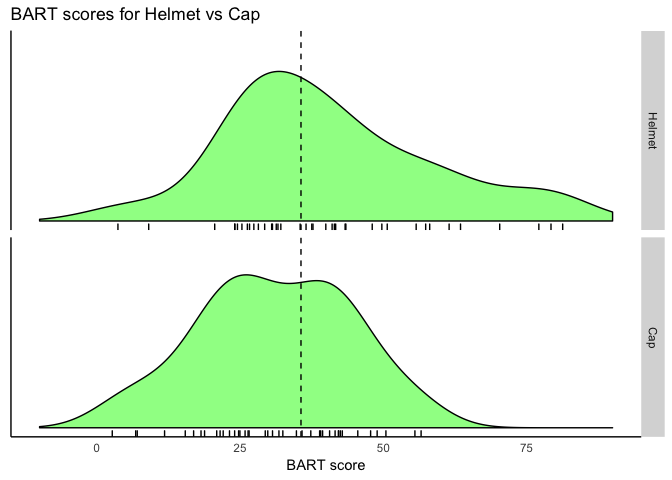
\includegraphics{hw_01_files/figure-latex/unnamed-chunk-7-1.pdf}

\begin{Shaded}
\begin{Highlighting}[]
\KeywordTok{ggplot}\NormalTok{(helmet, }\KeywordTok{aes}\NormalTok{(BART)) }\OperatorTok{+}
\StringTok{  }\KeywordTok{geom_density}\NormalTok{(}\DataTypeTok{fill=}\StringTok{"green"}\NormalTok{, }\DataTypeTok{alpha=}\NormalTok{.}\DecValTok{5}\NormalTok{)}\OperatorTok{+}
\StringTok{  }\KeywordTok{geom_rug}\NormalTok{()}\OperatorTok{+}
\StringTok{  }\KeywordTok{geom_vline}\NormalTok{(}\KeywordTok{aes}\NormalTok{(}\DataTypeTok{xintercept=}\KeywordTok{mean}\NormalTok{(helmet}\OperatorTok{$}\NormalTok{BART)))}\OperatorTok{+}
\StringTok{  }\KeywordTok{labs}\NormalTok{(}\DataTypeTok{title =} \StringTok{"a"}\NormalTok{, }\DataTypeTok{subtitle =} \StringTok{"Helmet"}\NormalTok{, }\DataTypeTok{x =} \StringTok{"Score"}\NormalTok{, }\DataTypeTok{y =} \StringTok{""}\NormalTok{)}\OperatorTok{+}
\StringTok{  }\KeywordTok{geom_vline}\NormalTok{(}\KeywordTok{aes}\NormalTok{(}\DataTypeTok{xintercept=}\FloatTok{35.6165}\NormalTok{), }\DataTypeTok{linetype=}\StringTok{"dashed"}\NormalTok{)}\OperatorTok{+}
\StringTok{  }\KeywordTok{ylim}\NormalTok{(}\KeywordTok{c}\NormalTok{(}\DecValTok{0}\NormalTok{,.}\DecValTok{06}\NormalTok{))}\OperatorTok{+}\KeywordTok{xlim}\NormalTok{(}\KeywordTok{c}\NormalTok{(}\OperatorTok{-}\DecValTok{20}\NormalTok{,}\DecValTok{100}\NormalTok{))}\OperatorTok{+}
\StringTok{  }\KeywordTok{theme}\NormalTok{(}\DataTypeTok{panel.grid.major =} \KeywordTok{element_blank}\NormalTok{(), }\DataTypeTok{panel.grid.minor =} \KeywordTok{element_blank}\NormalTok{(),}
\DataTypeTok{panel.background =} \KeywordTok{element_blank}\NormalTok{(), }\DataTypeTok{axis.line =} \KeywordTok{element_line}\NormalTok{(}\DataTypeTok{colour =} \StringTok{"black"}\NormalTok{),}\DataTypeTok{axis.text.y=}\KeywordTok{element_blank}\NormalTok{(),}
          \DataTypeTok{axis.ticks=}\KeywordTok{element_blank}\NormalTok{(),}
          \DataTypeTok{axis.title.y=}\KeywordTok{element_blank}\NormalTok{())}
\end{Highlighting}
\end{Shaded}

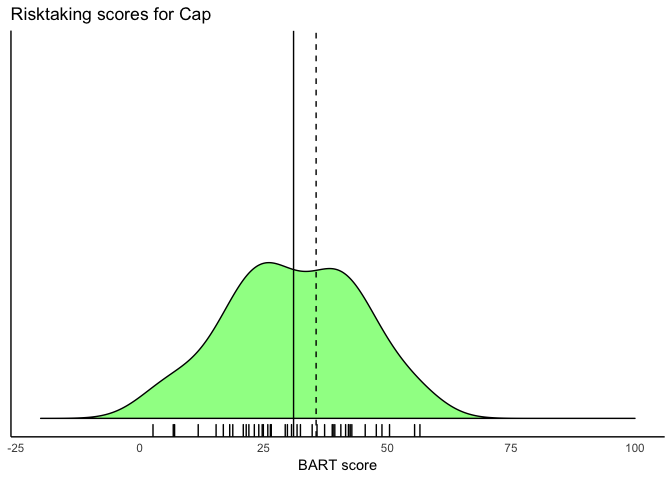
\includegraphics{hw_01_files/figure-latex/unnamed-chunk-7-2.pdf}

\begin{Shaded}
\begin{Highlighting}[]
\CommentTok{#plot b}
\CommentTok{#ggplot(bicycle, aes(SSS_total))+}
 \CommentTok{# facet_grid(Condition~.)+}
  \CommentTok{# geom_density(fill="green", alpha = .5)+}
 \CommentTok{# geom_rug() +}
 \CommentTok{# labs(title = "SSS scores for Helmet vs Cap", x = "SSS score", y = "")+}
 \CommentTok{#  ylim(c(0,.08))+xlim(c(0,40))+}
 \CommentTok{# geom_vline(aes(xintercept=mean(SSS_total)), linetype = "dashed")+}
 \CommentTok{# theme(panel.grid.major = element_blank(), panel.grid.minor = element_blank(),}
\CommentTok{#panel.background = element_blank(), axis.line = element_line(colour = "black"),axis.text.y=element_blank(),}
        \CommentTok{#  axis.ticks=element_blank(),}
         \CommentTok{# axis.title.y=element_blank())}

\KeywordTok{ggplot}\NormalTok{(hat, }\KeywordTok{aes}\NormalTok{(SSS_total)) }\OperatorTok{+}
\StringTok{  }\KeywordTok{geom_density}\NormalTok{(}\DataTypeTok{fill=}\StringTok{"green"}\NormalTok{, }\DataTypeTok{alpha =}\NormalTok{ .}\DecValTok{5}\NormalTok{)}\OperatorTok{+}
\StringTok{  }\KeywordTok{geom_rug}\NormalTok{() }\OperatorTok{+}
\StringTok{  }\KeywordTok{labs}\NormalTok{(}\DataTypeTok{title =}\StringTok{"b"}\NormalTok{, }\DataTypeTok{subtitle=}  \StringTok{"Cap"}\NormalTok{, }\DataTypeTok{x =} \StringTok{"SSS score"}\NormalTok{, }\DataTypeTok{y =} \StringTok{""}\NormalTok{)}\OperatorTok{+}
\StringTok{   }\KeywordTok{ylim}\NormalTok{(}\KeywordTok{c}\NormalTok{(}\DecValTok{0}\NormalTok{,.}\DecValTok{1}\NormalTok{))}\OperatorTok{+}\KeywordTok{xlim}\NormalTok{(}\KeywordTok{c}\NormalTok{(}\DecValTok{0}\NormalTok{,}\DecValTok{40}\NormalTok{))}\OperatorTok{+}
\StringTok{  }\KeywordTok{geom_vline}\NormalTok{(}\KeywordTok{aes}\NormalTok{(}\DataTypeTok{xintercept=}\KeywordTok{mean}\NormalTok{(hat}\OperatorTok{$}\NormalTok{SSS_total)))}\OperatorTok{+}
\StringTok{  }\KeywordTok{geom_vline}\NormalTok{(}\KeywordTok{aes}\NormalTok{(}\DataTypeTok{xintercept=}\FloatTok{20.95}\NormalTok{), }\DataTypeTok{linetype =} \StringTok{"dashed"}\NormalTok{)}\OperatorTok{+}
\StringTok{  }\KeywordTok{theme}\NormalTok{(}\DataTypeTok{panel.grid.major =} \KeywordTok{element_blank}\NormalTok{(), }\DataTypeTok{panel.grid.minor =} \KeywordTok{element_blank}\NormalTok{(),}
\DataTypeTok{panel.background =} \KeywordTok{element_blank}\NormalTok{(), }\DataTypeTok{axis.line =} \KeywordTok{element_line}\NormalTok{(}\DataTypeTok{colour =} \StringTok{"black"}\NormalTok{),}\DataTypeTok{axis.text.y=}\KeywordTok{element_blank}\NormalTok{(),}
          \DataTypeTok{axis.ticks=}\KeywordTok{element_blank}\NormalTok{(),}
          \DataTypeTok{axis.title.y=}\KeywordTok{element_blank}\NormalTok{())}
\end{Highlighting}
\end{Shaded}

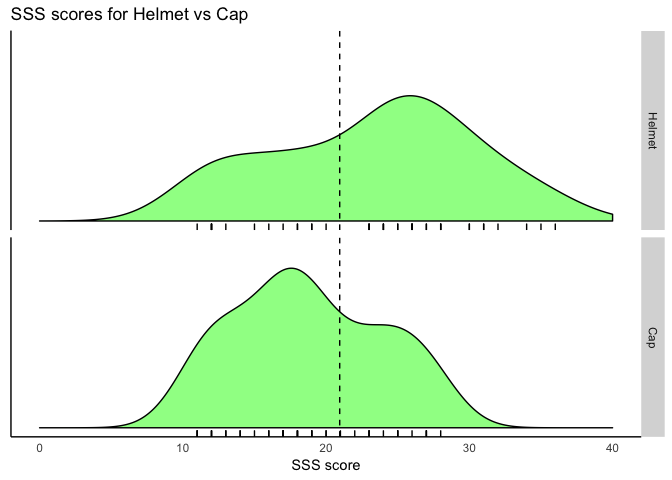
\includegraphics{hw_01_files/figure-latex/unnamed-chunk-8-1.pdf}

\begin{Shaded}
\begin{Highlighting}[]
\KeywordTok{ggplot}\NormalTok{(helmet, }\KeywordTok{aes}\NormalTok{(SSS_total)) }\OperatorTok{+}
\StringTok{  }\KeywordTok{geom_density}\NormalTok{(}\DataTypeTok{fill=}\StringTok{"green"}\NormalTok{, }\DataTypeTok{alpha=}\NormalTok{.}\DecValTok{5}\NormalTok{)}\OperatorTok{+}
\StringTok{  }\KeywordTok{geom_rug}\NormalTok{()}\OperatorTok{+}
\StringTok{  }\KeywordTok{labs}\NormalTok{(}\DataTypeTok{title =}\StringTok{"b"}\NormalTok{, }\DataTypeTok{subtitle =}  \StringTok{"Helmet"}\NormalTok{, }\DataTypeTok{x =} \StringTok{"SSS score"}\NormalTok{, }\DataTypeTok{y =} \StringTok{""}\NormalTok{) }\OperatorTok{+}
\StringTok{   }\KeywordTok{ylim}\NormalTok{(}\KeywordTok{c}\NormalTok{(}\DecValTok{0}\NormalTok{,.}\DecValTok{1}\NormalTok{))}\OperatorTok{+}\KeywordTok{xlim}\NormalTok{(}\KeywordTok{c}\NormalTok{(}\DecValTok{0}\NormalTok{,}\DecValTok{50}\NormalTok{))}\OperatorTok{+}
\StringTok{  }\KeywordTok{geom_vline}\NormalTok{(}\KeywordTok{aes}\NormalTok{(}\DataTypeTok{xintercept=}\KeywordTok{mean}\NormalTok{(helmet}\OperatorTok{$}\NormalTok{SSS_total)))}\OperatorTok{+}
\StringTok{    }\KeywordTok{geom_vline}\NormalTok{(}\KeywordTok{aes}\NormalTok{(}\DataTypeTok{xintercept=}\FloatTok{20.95}\NormalTok{), }\DataTypeTok{linetype=}\StringTok{"dashed"}\NormalTok{)}\OperatorTok{+}
\StringTok{  }\KeywordTok{theme}\NormalTok{(}\DataTypeTok{panel.grid.major =} \KeywordTok{element_blank}\NormalTok{(), }\DataTypeTok{panel.grid.minor =} \KeywordTok{element_blank}\NormalTok{(),}
\DataTypeTok{panel.background =} \KeywordTok{element_blank}\NormalTok{(), }\DataTypeTok{axis.line =} \KeywordTok{element_line}\NormalTok{(}\DataTypeTok{colour =} \StringTok{"black"}\NormalTok{),}\DataTypeTok{axis.text.y=}\KeywordTok{element_blank}\NormalTok{(),}
          \DataTypeTok{axis.ticks=}\KeywordTok{element_blank}\NormalTok{(),}
          \DataTypeTok{axis.title.y=}\KeywordTok{element_blank}\NormalTok{()) }
\end{Highlighting}
\end{Shaded}

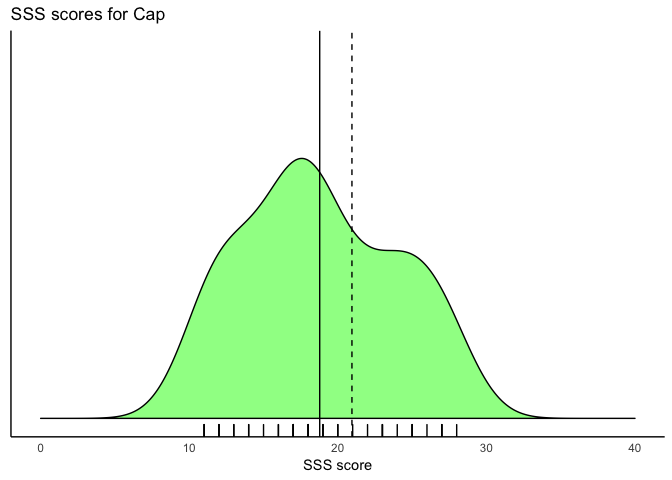
\includegraphics{hw_01_files/figure-latex/unnamed-chunk-8-2.pdf}


\end{document}
